\section{my\-Dialog::Load\-FITSFile\-Dialog Class Reference}
\label{classmyDialog_1_1LoadFITSFileDialog}\index{myDialog::LoadFITSFileDialog@{myDialog::LoadFITSFileDialog}}
Inheritance diagram for my\-Dialog::Load\-FITSFile\-Dialog::\begin{figure}[H]
\begin{center}
\leavevmode
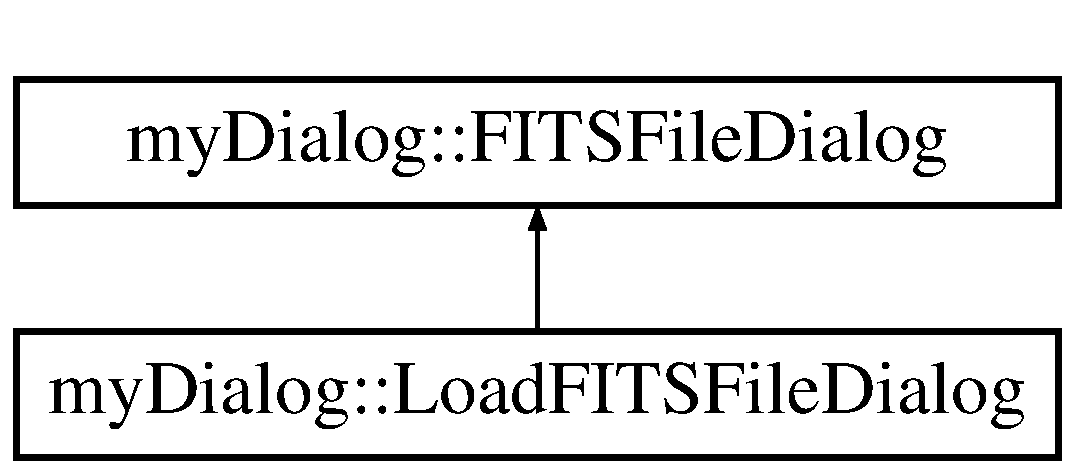
\includegraphics[height=2cm]{classmyDialog_1_1LoadFITSFileDialog}
\end{center}
\end{figure}
\subsection*{Public Member Functions}
\begin{CompactItemize}
\item 
def \textbf{ok\_\-command}\label{classmyDialog_1_1LoadFITSFileDialog_f56aa086e9e143266c0d4f1a080c4bae}

\item 
def \textbf{set\_\-selection}\label{classmyDialog_1_1LoadFITSFileDialog_9af3c30e2ad0e5ca3e4d35da2a8276a7}

\end{CompactItemize}
\subsection*{Static Public Attributes}
\begin{CompactItemize}
\item 
string \textbf{title} = \char`\"{}Select file\char`\"{}\label{classmyDialog_1_1LoadFITSFileDialog_ed814de16cb771269b0cbc1dc9723abe}

\end{CompactItemize}


\subsection{Detailed Description}


\footnotesize\begin{verbatim}File selection dialog which checks that the file exists.\end{verbatim}
\normalsize
 



The documentation for this class was generated from the following file:\begin{CompactItemize}
\item 
old/PANICtool-1.0/my\-Dialog.py\end{CompactItemize}
